\section{MARCO TEÓRICO}

El objetivo de este capítulo es presentar los aspectos teóricos de esta tesis sobre D-Minute como un artefacto del diálogo para mejorar las reuniones de proyectos. En primer lugar, se establecen los elementos conceptuales necesarios para entender el problema y la solución del \textit{software}. Más adelante, se describen los fundamentos teóricos para situar el contexto del problema. En segundo lugar, se presenta el estado del arte que presenta una revisión actualizada de la literatura sobre \textit{meetingware}. Por último, el marco de investigación que guía el desarrollo de la tesis.

\subsection{SITUACIÓN \textit{MEETINGWARE}}

\textit{Meetingware} es un área que apoya, gestiona, orienta y estimula la participación en reuniones  \cite{RN7}, a su vez es un interlocutor de diferentes actores que participan en el desarrollo de esta instancia, como son: personas, \textit{hardware, software y roomware} \cite{RN7}. Esto es debido a que las reuniones son un sitio para el trabajo colectivo, una de las principales formas en que las empresas aprovechan la diversidad de opiniones, el entendimiento común y la resolución de problemas \cite{RN25}. Las reuniones son definidas como el lugar para estructurar y coordinar el trabajo de la organización, esta explicación se debe a que avanzamos hacia una economía basada en el conocimiento, pues la diversidad de información permite la correcta toma de decisiones y el éxito de un determinado proyecto dentro de la organización \cite{RN7} que impactaría positivamente el resultado de esta. Sin más, las reuniones son instancias relevantes dentro de la coordinación de un trabajo, sin embargo, se hace difícil conseguir que las personas coincidan en tiempo y espacio físico a estas instancias a consecuencia de las actividades que tiene cada persona del equipo y es por ello que han surgido: reuniones virtuales \cite{RN23}, reuniones diarias \cite{RN35}, reuniones específicas y reuniones ordinarias o recurrentes \cite{RN25}. Esto ha permitido al área de \textit{meetingware} realizar el desarrollo de herramientas que apoyen esta labor \cite{RN28}, pues los impactos de reuniones son significativos para una empresa por la gran cantidad de horas que las personas pasan en ellas, los recursos críticos no movilizados y los costos de oportunidad involucrados.

\subsection{ARTEFACTO DEL DIÁLOGO}

La teoría de diálogo/acción \fullcite{RN24} postula una plataforma como un terreno común para alojar las conversaciones abiertas y colaborativas que mantienen los equipos, ver figura \ref{img2-1}. Esta es una propuesta en la cual se detalla que el diálogo está conformado por cuatro aspectos cognitivos básicos denominados elementos o síntesis del dialógicos. Estos elementos están relacionados con la estabilidad y el cambio en el diálogo; los acuerdos y compromisos establecen la estabilidad o convergencia de puntos de vista, las dudas y los desacuerdos establecen el cambio o la divergencia de opiniones.

\begin{figure}[h]
\centering
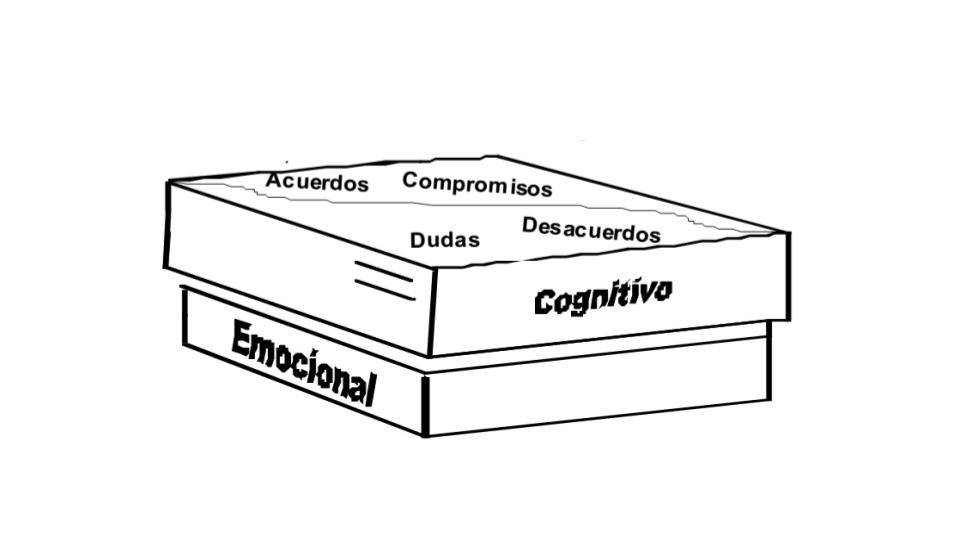
\includegraphics[width=0.7\linewidth]{/img2-1}
\caption{Plataforma del diálogo, tomado de (Leiva-Lobos, Antillanca y Ponce, 2008)} 
\label{img2-1}
\end{figure}

Aunque la dimensión emocional de los participantes en una conversación no se aborda en esta tesis; es preciso destacar que si no se generan las emociones adecuadas en una reunión, sencillamente el diálogo no ocurre. Además, es importante destacar que los componentes de la plataforma del diálogo mantienen y permiten llevar a una trayectoria histórica de la conversación que se puede seguir y gestionar.

Los elementos que componen la plataforma del diálogo y su descripción son los siguientes:

\begin{itemize}
	\item \textbf{Dudas (du):} Se plantea falta de información sobre un tema particular o no existe claridad sobre el problema, la oportunidad o las alternativas de solución. Esto crea incertidumbre en cómo continuar con el proyecto. Por ejemplo: “¿Qué tecnología es la más apropiada para este proyecto?”.
	\item \textbf{Desacuerdos (de):} Se presenta una contraposición entre puntos de vista sobre un tema o se detecta una brecha entre lo proyectado versus lo logrado. En ambos casos es necesario resolver el asunto para continuar el proyecto. Por ejemplo: “¡El proyecto será un éxito!,  yo no estaría tan confiado como tú”.
	\item \textbf{Compromiso (co):} Ciertos compromisos deben ser asumidos por personas específicas en fechas específicas para asegurarse que se realicen. Ni las reglas ni los acuerdos de coordinación colectivos logran ese efecto.  Por ejemplo: “Me comprometo que para la próxima reunión resolveré el problema del navegador chrome para funcione nuestro plug-in”.
	\item \textbf{Acuerdo (ac):} La coordinación grupal requiere acuerdos asumidos por todos. Si no son normas comunes o compromisos individuales se deben tratar como acuerdos de coordinación.  Por ejemplo: “Las reuniones diarias serán a las 12 pm”.

\end{itemize}

Si observamos los puntos anteriores nos podemos percatar que cada elemento conlleva una actividad y estas deben estar basadas en un parámetro común para todos pues el diálogo solo se puede generar si estamos dentro del mismo contexto conversacional \fullcite{RN34},  por favor observar la siguiente la figura \ref{img2-2}.

\begin{figure}[h]
\centering
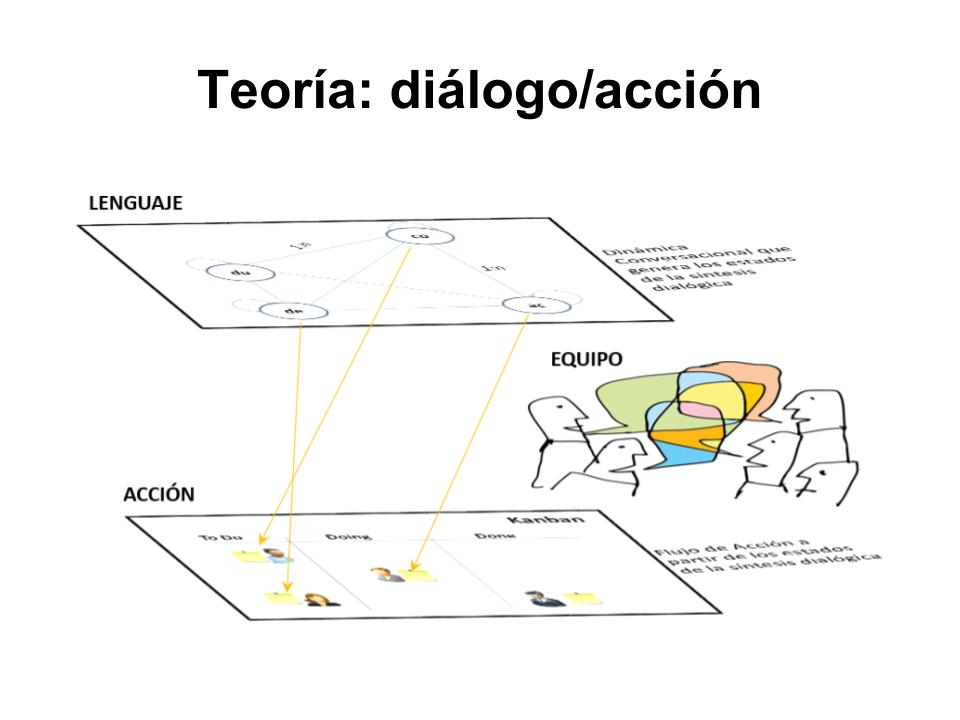
\includegraphics[width=0.7\linewidth]{/MetodoReunionesAgiles}
\caption{Articulación entre el plano del lenguaje y el plano de la acción que promociona el enfoque diálogo/acción, elaboración propia} 
\label{img2-2}
\end{figure}

Los acuerdos son declaraciones o reglas que fijan comportamientos humanos colectivos. Si son trascendentes para la demarcación del proyecto se llama “norma común”. Si esos acuerdos no fijan “una ley” permanente son consensos operativos se llaman “acuerdos de coordinación”. Por otro lado, para que se pase de los elementos del diálogo a la acción aparece un nuevo elemento denominado “tarea” (ta). Ahora, se identifican de manera más precisa estos tres elementos con las siguientes definiciones:

\begin{itemize}
	\item \textbf{Norma común:} La falta de normas, reglas o estándares comunes producen caos. Las normas y reglas comunes ordenan el trabajo. Estas reglas deben ser aceptadas colectivamente y consideradas leyes para operar en el futuro en el contexto del proyecto colectivo que se lleva a cabo. Por ejemplo: “Desde ahora en adelante usaremos solo metodologías Lean para proyectos pequeños”.
	\item \textbf{Acuerdos de coordinación:} Cuando no se trata de una regla o norma común y se precisa una coordinación en la acción se establecen por descarte este tipo de acuerdos. Por ejemplo, “Mañana a las 9 todos aquí”.
	\item \textbf{Tarea (ta):} Acción emprendida por una persona para lograr un objetivo. Aunque es obvio que un compromiso da lugar a una tarea. Resolver desacuerdos, resolver dudas, implementar normas, o la coordinación grupal dan origen a nuevas tareas. Luego se puede ir desde el conjunto (ac, de, du, co) a la tarea (ta). Un ejemplo de tarea es el siguiente: “Reparar el plug-in prometido en la reunión seis para las 12 am del jueves”.
\end{itemize}

Los elementos del dialog descritos, son representados por los iconos expuestos en imagen \ref{img2-3}

\begin{figure}[h]
\centering
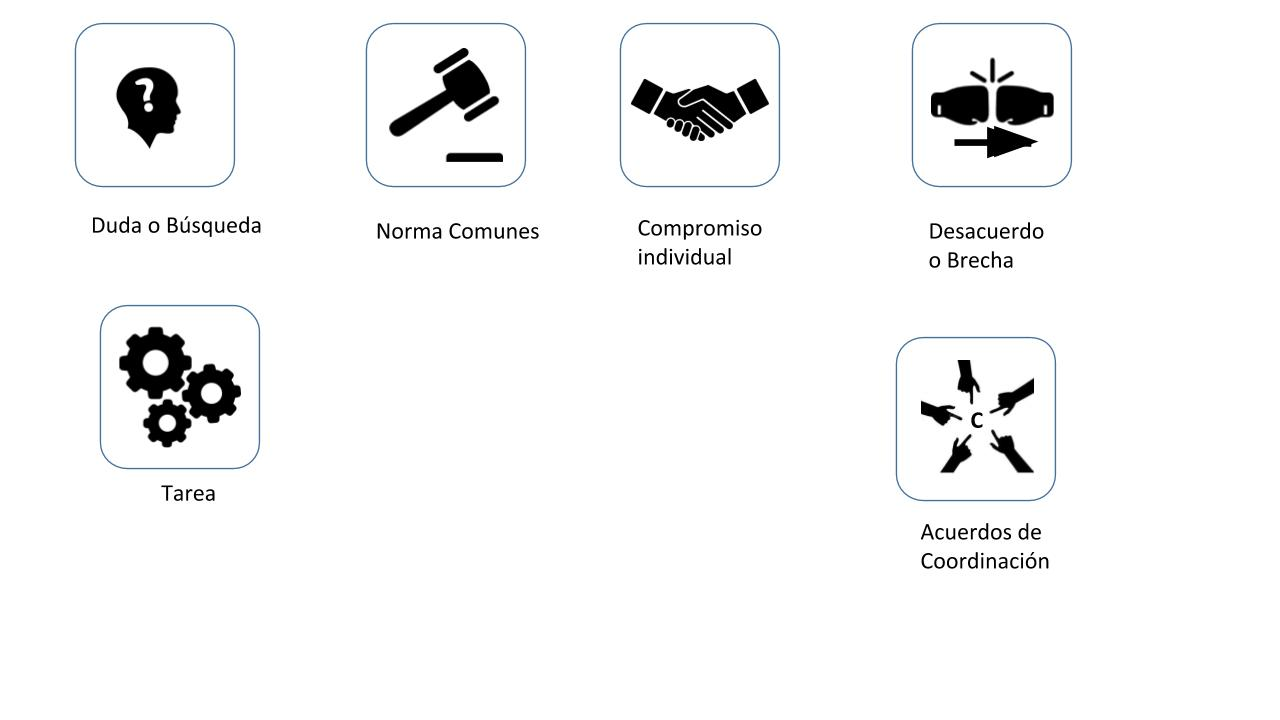
\includegraphics[width=0.7\linewidth]{/IconosDialogo-Accion}
\caption{Iconografía elementos del diálogo, elaboración propia} 
\label{img2-3}
\end{figure}

\subsection{ESTADO DEL ARTE}

Las reuniones y su efecto en las personas han sido analizadas por diferentes áreas del conocimiento: \textit{Knowledge Management, Dialogue, Collective Intelligence, Computer Supported Cooperative Work, Contested Collective Intelligence, meetingware}, por nombrar algunas; durante varias décadas han buscado que la comunicación, la coordinación, la cooperación sean parte integral de un flujo de trabajo colaborativo en reuniones del tipo \textit{co-located} síncrono y asíncrono, mediante el uso eficiente de la tecnología.

En 1970 Rittel y Kunz - citado por \fullcite{RN19} - publican \textit{Issue-Based Information System} (IBIS) un sistema para la captura de puntos esenciales en la discusión de problemas. Su notación se compone de: problemas (lo que se desea abordar), posiciones (las respuestas al problema) y argumentos (pros y contras de un problema), en 1988 Conklin y Begeman - citado por \fullcite{RN19} - adoptan el sistema para su uso en computadores, luego derivó a una variante para el mapeo de las conversaciones que se da en reuniones informales, para mejorar la inclusión de la discusión \fullcite{RN19}.

En 1986 Daft y Lengel - citado por \fullcite{RN21} - distinguen dos tipos de confusión que la gente puede tener con un elemento de discusión: la ambig\"uedad y la incertidumbre. Con esta distinción \fullcite{RN21} indican que las reuniones de decisión pueden considerarse como una composición de una parte divergente y una convergente. Proponen PRIME basado la notación de IBIS para el apoyo de reuniones de decisión y a su parte divergente de la discusión. Dicha parte que puede ser llamada “desacuerdo” relacionada con el cambio, en base a la teoría del diálogo propuesta el mismo año por \fullcite{RN24} donde postulan cuatro aspectos cognitivos que forman parte de la plataforma del diálogo, dos relacionados con la estabilidad: \textbf{acuerdo} al que se llega y \textbf{compromiso} que se toma (y quienes los toman); y dos relacionados con el cambio: \textbf{duda} que se genera al hablar de un tema y \textbf{desacuerdo} que se provoca cuando hay divergencia de opiniones. Esta teoría establece tres principios para el diálogo: apertura, continuidad y simetría. En particular, para ayudar a la continuidad del diálogo se conceptualiza un artefacto tangible denominado "Acta Dialógica" de allí el nombre del artefacto que se presenta en esta tesis D-Minute (\textit{Dialogic Minute}). A través de esta herramienta se pretende seguir la traza y el estado de los elementos que son parte de la plataforma del diálogo.

Chang, Liou Huang, Yu \& Shiah (1999) se mueven a la línea de \textit{co-located} asíncrono y proponen un sistema de minutas de conferencia basado en la \textit{World Wide Web} permitiendo tener hipervínculos de toda la información del proyecto, contener la memoria de la organización de este y que pueda ser heredada a nuevos participantes.

Volviendo a la línea \textit{co-located} síncrono \fullcite{RN37} presentan CollabMeet, un sistema de captura de información de reuniones basada en teléfono móvil, donde los participantes graban momentos importantes de la discusión, esto ayuda a minimizar las interrupciones y la distracción cuando la reunión es muy intensa. En una siguiente reunión pueden recurrir a la temática grabada en la reunión pasada para recuperar y re-situarse en el contexto del proyecto.

De Liddo \& Buckingham Shum (2010) exponen el modelo conceptual de Cohere, una plataforma hipermedia para investigación que permite explorar las nuevas ideas, apunta al concepto de inteligencia colectiva donde personas y grupos crean ideas en un entorno web. Ofrece seguimiento para las interpretaciones más allá si estas convergen o divergen entre sus participantes. Esto a su vez y en un área diferente pero no lejana se encuentra relacionado con la estabilidad o convergencia (acuerdo, compromiso) y el cambio o divergencia (desacuerdo, dudas) de la plataforma del diálogo propuesto en \fullcite{RN24}. Cohere además, se basa en IBIS para el mapeo de argumentos estructurados que se dan en las ideas expuestas por el grupo.

Bossel (2012) toma la teoría del diálogo de \fullcite{RN24} y genera un prototipo en papel de minuta que permita a un equipo reconectar y explorar la memoria colectiva del proyecto en base a reuniones periódicas, siguiendo la teoría del diálogo/acción.

En 2014 surgieron trabajos en la Universidad de Chile, que adoptaron el prototipo de minuta propuesto por \fullcite{RN14}, desarrollaron una aplicación web que facilita la continuidad y recuperación de los elementos del diálogo \fullcite{RN42} y que fue continuado por \fullcite{RN41} en su memoria de ingeniería civil en informática. Lamentablemente, ambos prototipos poseen demasiados problemas de usabilidad para ser considerados en una prueba de concepto robusta de las ideas de acta dialógica.

Por otra parte, sabemos que las reuniones son esenciales para coordinar y estructurar el trabajo, pero se estima que muchas de las herramientas desarrolladas en CSCW o groupware carecen de resultados en la práctica \fullcite{RN17} debido a que no son evaluadas de manera formal por los investigadores \fullcite{RN38}. Este punto es sumamente importante para la generación de un artefacto tecnológicos eficiente y usable y sobre todo válido.

Antunes \& Carrio (2003) proponen: Modelo de estructuras para reuniones, en el cual se identifican tres elementos fundamentales: (1) roles, abordando la diversidad de personas y actividades; (2) recursos, teniendo en cuenta la logística de la reunión y (3) proceso, dirigiéndose a la organización del conjunto de actividades.

En la misma línea Antunes \& Costa (2003) proponen: Perceived Value, un método para evaluar \textit{Meetingware} por medio de diferentes atributos respecto a una medida de costos y beneficios. Estos atributos son contribuciones que se dan por tres factores: individual, grupo y organización, básicamente porque el éxito o el fracaso depende de su combinación. Se organizan tres columnas, la primera se refiere a los roles, la segunda aborda el proceso de una reunión y la tercera para caracterizar el cumplimiento de los recursos donde la votación se limita a 0 para “no ayuda” y 1 “ayuda”, donde su “valor percibido” es calculado mediante una ecuación matemática, dicho valor debe ser mayor a la media (45). Siendo este resultado una medida para decidir si es válido continuar con la reunión. \fullcite{RN28} siguiendo una línea similar, describen el desarrollo y prueba de un instrumento para evaluar las reuniones por medio de un conjunto de factores de entrada, de proceso y resultado. Donde el primer paso de la evaluación es conocer el comportamiento en un marco de reuniones de proyecto y en segundo lugar medir los factores (evaluación, cuestionarios, etc), para determinar si el instrumento es confiable y útil para el apoyo a las reuniones.

Dhenesh, Sitnikova \& Slay (2012) para guiar la creación de herramientas, generan lecciones para el desarrollo de un sistema integrado que apoye las reuniones de trabajo y donde la adopción de la herramienta por los participantes sea inclusiva, debido a que muchas herramientas fallan en la práctica en incorporar esta característica.

\subsection{MARCO DE LA INVESTIGACIÓN DE MERCADO}

En este punto se formula cuál será el marco de investigación asociado a la innovación (la “i” chica en “I+D+i”) y desarrollo que guía este estudio. Se proponen las preguntas de investigación que se van a someter a análisis.

En la revisión bibliográfica realizada, las herramientas de \textit{meetingware} no poseen al menos las siguientes características que:

\begin{enumerate}[1.]
    \item Aplique elementos que sinteticen la convergencia y la divergencia de argumentos de manera explícita
    \item Exponga las tareas de forma visual.
    \item Permita recorrer las reuniones anteriores con flexibilidad y pertinencia.
    \item Permite editar los elementos del hilo argumental de la reunión y que son fruto de las discusiones al interior del equipo de desarrollo. En el caso de la teoría de diálogo/acción son los acuerdos, desacuerdos, dudas y compromisos.
\end{enumerate}

En base al estado del arte, se evidencia que existen herramientas que utilizan uno o alguno de los elementos del diálogo expuestos por \fullcite{RN24}. Sin embargo, los enfoques en los \textit{meetingware} desarrollados son distintos pero no alejados puesto que muchos conducen a una generación de diálogo. Esto propone las siguientes preguntas de investigación de mercado:

\begin{enumerate}[1.]
    \item ¿D-Minute expone los argumentos del diálogo y su seguimiento mejor que otras herramientas síncronas co-locadas de la investigación?
    \item ¿Qué ventaja competitiva posee D-Minute respecto a los productos comerciales existentes hoy día en el mercado?
\end{enumerate}

\subsection{RESUMEN}

El presente capítulo expone la revisión de la literatura que dan fundamento al desarrollo de esta tesis, situando en el contexto de \textit{meetingware} el trabajo realizar. Debido a que en esta línea de investigación es donde existe el mayor desarrollo de herramientas para el apoyo de reuniones, además de variados estudios que permiten medir la efectividad de las herramientas desarrolladas. 

En este trabajo y por medio de la plataforma del diálogo se busca determinar la efectividad que puede tener D-Minute -\textit{software} a desarrollar para la validación de la hipótesis- en comparación a otras herramientas del mercado. Es importante mencionar que D-Minute será la evolución del proyecto desarrollado en la Universidad de Chile por \fullcite{RN42} y la de \fullcite{RN41}.

Para este trabajo se va seleccionar herramientas del mercado que sirvan de apoyo a la reuniones de trabajo con el fin de establecer criterios de evaluación que permitan medir D-Minute con sus competidores es preciso leer el capítulo 3.
